\documentclass[11pt]{beamer}
\usefonttheme[onlymath]{serif}

\setbeamersize{text margin left=1.5em}
\setbeamersize{text margin right=1.5em}




\setbeamertemplate{frametitle}{%
  \vskip1ex
  \usebeamerfont{frametitle}%
  \insertframetitle\par %frame 에서 지정한 title 사용
  %\insertsubsectionhead\par        % subsection의 header를 사용
  \vskip1ex
  \hrule                             % 밑줄(선택)
}

\setbeamertemplate{blocks}[rounded][shadow=true] % 블록 테두리 둥글게

\setbeamertemplate{itemize item}{\usebeamerfont{itemize item}\textbullet}
\setbeamertemplate{itemize subitem}{\usebeamerfont{itemize subitem}\textbullet}
\setbeamertemplate{itemize subsubitem}{\usebeamerfont{itemize subsubitem}\textbullet}



%\setbeamerfont{itemize/enumerate subbody}{parent=itemize/enumerate body} % 
%\setbeamerfont{itemize/enumerate subbody}{size=\usebeamerfont{itemize/enumerate body}\size}

\makeatletter
% Taken from beamer.cls' default geometry settings
% http://mirrors.ctan.org/macros/latex/contrib/beamer/base/beamer.cls
\geometry{%
  papersize={\fpeval{\beamer@paperwidth*1.5}pt,\fpeval{\beamer@paperheight*1.5}pt},
  hmargin=\fpeval{0.5 * 1.5}cm,% 1cm
  vmargin=0cm,%
  head=\fpeval{0.5*1.5}cm,% 0.5cm
  headsep=0pt,%
  foot=\fpeval{0.5*1.5}cm% 0.5cm
}
\makeatother %from search keyword beamer size, get this search result -> https://tex.stackexchange.com/questions/586756/beamer-use-glyphs-from-smaller-font-size-but-enlarge


% Reference bibtex
% style = numeric, apa, authoryear-comp
\usepackage[backend=biber, style=authoryear-comp, natbib=true]{biblatex}
\addbibresource{../../references.bib}



% 테마 선택 (선택 사항)
% \usetheme{Madrid} % 기본 테마, 다른 테마 사용 가능
% \font{serif}
\usepackage{amsfonts}
\usepackage{amssymb}
\usepackage[T1]{fontenc} % To use combination of textbf, textit
\usepackage[dvipsnames]{xcolor}   % can use more variant colors
%\usepackage{lmodern} %다른 폰트 사용: 문서의 서문에 추가하면 Computer Modern 폰트의 확장 버전인 Latin Modern 폰트를 사용할 수 있습니다. 이 폰트는 더 다양한 크기와 스타일을 지원하여 문제를 해결해 줄 수 있습니다.

% \setcounter{MaxMatrixCols}{20}

% (필요한 패키지들)
% \usepackage{amsthm}
\setbeamertemplate{theorems}[numbered]  % 정리, 정의 등에 번호를 달아줌

% \theoremstyle{plain} % insert bellow all blocks you want in italic
% \newtheorem{theorem}{Theorem}[section] % to number according to section
% 
% \theoremstyle{definition} % insert bellow all blocks you want in normal text
% \newtheorem{definition}{Definition}[section] % to number according to section
% \newtheorem*{idea}{Proof idea} % no numbered block

\newtheorem{proposition}[theorem]{Proposition}

\usepackage{tcolorbox}

% 필요할 경우 패키지 추가
\usepackage{graphicx} % 이미지 삽입을 위한 패키지
\usepackage{amsmath}   % 수식 사용
\usepackage{hyperref}  % 하이퍼링크 추가
\hypersetup{
  colorlinks=true,
  linkcolor=blue,
} % search keyword: beamer hyperref color -> https://tex.stackexchange.com/questions/13423/how-to-change-the-color-of-href-links-for-real
%search keyword: hyperref color -> https://www.overleaf.com/learn/latex/Hyperlinks
\usepackage{cleveref}
\usepackage{multicol}  % 여러 열 나누기
\usepackage{ulem} % 취소선 및줄 나누기
\usepackage{mathtools} % dcases
%\usepackage{xparse} % NewDocumentCommand
\usepackage[boxed, lined]{algorithm2e} % to use algorithm block



% \NewDocumentCommand{\DefThreeOp}{m}{%
%   % \csname #1\endcsname 라는 이름으로, 3개 인자를 받는 새 매크로를 정의
%   \expandafter\NewDocumentCommand\csname #1\endcsname{mmm}{%
%     \operatorname{#1}\!\bigl(##1,\,##2,\,##3\bigr)%
%   }%
% }

\newcommand{\mrm}[1]{\mathrm{#1}}
\newcommand{\mbb}[1]{\mathbb{#1}}
\newcommand{\mb}[1]{\mathbf{#1}}
\newcommand{\mc}[1]{\mathcal{#1}}
\newcommand{\tb}[1]{\textbf{#1}}
\newcommand{\ti}[1]{\textit{#1}}
\newcommand{\Pois}[1]{\operatorname{Pois}(#1)}

\newcommand{\myber}[1]{\operatorname{Bern}\!\left(#1\right)}
\newcommand{\Bin}[2]{\operatorname{Bin}\!\left(#1,#2\right)}
\newcommand{\NBin}[2]{\operatorname{NBin}\!\left(#1,#2\right)}
\newcommand{\mytoinf}[1]{#1 \rightarrow \infty}
\newcommand{\myexp}[1]{\exp{\left(#1\right)}}
\newcommand{\Unif}[2]{\operatorname{Unif}\!\left(#1, #2\right)}
\newcommand{\UnifOne}[1]{\operatorname{Unif}\!\left(#1\right)}
\newcommand{\mygeom}[1]{\operatorname{Geom}\!\left(#1\right)}
\newcommand{\Expo}[1]{\operatorname{Expo}\!\left(#1\right)}
\newcommand{\abs}[1]{\left\lvert #1 \right\rvert}
\newcommand{\floor}[1]{\left\lfloor #1 \right \rfloor}
\newcommand{\expec}[1]{\operatorname{E}\left[ #1 \right]}
\newcommand{\Var}[1]{\operatorname{Var}\left[#1\right]}
\newcommand{\myskew}[1]{\operatorname{Skew}\!\left[#1\right]}
\newcommand{\mykurt}[1]{\operatorname{Kurt}\!\left[#1\right]}
\newcommand{\mywei}[2]{\operatorname{Wei}\!\left(#1, #2\right)}
\newcommand{\Span}{\operatorname{Span}}
\newcommand{\Cov}[2]{\operatorname{Cov}\!\left(#1, #2\right)}
\newcommand{\intinfty}{\int_{-\infty}^\infty}
\newcommand{\Corr}[2]{\operatorname{Corr}\!\left(#1, #2\right)}
\newcommand{\Mult}[3]{\operatorname{Mult}_{#1}\!\left(#2, #3\right)}
\newcommand{\Beta}[2]{\operatorname{Beta}\!\left(#1, #2\right)}
\newcommand{\HGeom}[3]{\operatorname{HGeom}\!\left(#1, #2, #3\right)}
\newcommand{\NHGeom}[3]{\operatorname{NHGeom}\!\left(#1,#2, #3\right)}
\newcommand{\GammaDist}[2]{\operatorname{Gamma}\!\left(#1, #2\right)}
%\DefThreeOp{PHGeom}

\newcommand{\im}{\operatorname{im}}
\newcommand{\tr}{\operatorname{tr}}
\newcommand{\supp}{\operatorname{supp}}


% 발표 제목, 저자, 날짜 설정
\title{Offline Learing: Conservative Q-Learning (CQL)}
\author{Gwanwoo Choi}
% \date{}

\begin{document}
% 표지 슬라이드

\begin{frame}
    \titlepage
\end{frame}

% \begin{frame}{asdf}
%     \begin{itemize}
%         \item https://ella-jiwon.tistory.com/4
%     \end{itemize}
% \end{frame}

\begin{frame}{Offline Reinforcement Learning}
    Offline Reinforcement Learning: Learning policies from a pre-collected dataset without any further interaction with the environment.

    \begin{figure}
        \centering
        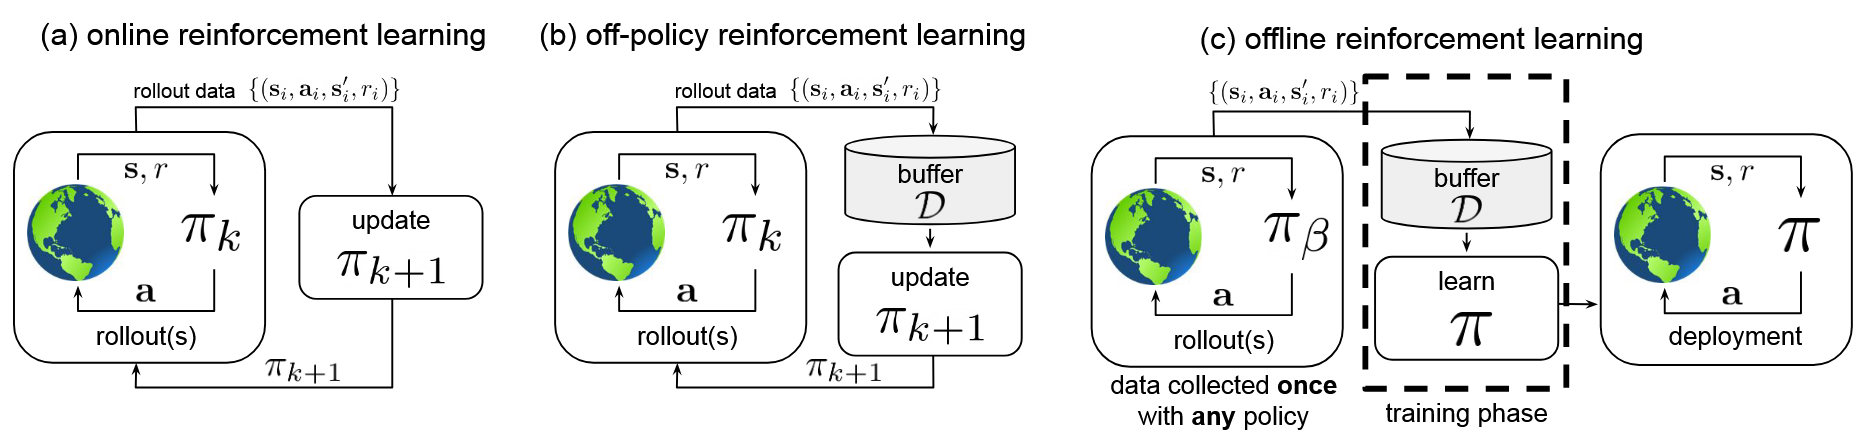
\includegraphics[width=0.95\textwidth]{OfflineRL.png}
    \end{figure}

    \begin{itemize}
        \item Online RL: The agent interacts with the environment and updates its policy directly using the most recent transition.
        \item Off-policy RL: The agent stores its encountered transitions in a replay buffer and updates its policy by sampling from this buffer.
        \item Offline RL: The agent learns a policy exclusively from a fixed, pre-collected dataset without any further interaction with the environment.
    \end{itemize}
\end{frame}

\begin{frame}{Preliminaries}
    MDP is defined by tuple $(\mc{S}, \mc{A}, T, r, \gamma)$
    \begin{itemize}
        \item State Space $\mc{S}$
        \item Action Space $\mc{A}$
        \item Transition Probability $T: \mc{S} \times \mc{A} \to \Delta(S)$
        \item Reward Function $r : \mc{S} \times \mc{A} \to [R_{\text{min}}, R_{\text{max}}]$
        \item Discount Factor : $\gamma \in [0,1)$
    \end{itemize}
    In Offline Reinforcement Learning, there exists
    \begin{itemize}
        \item Behavior Policy $\beta: \mc{S} \to \Delta(\mc{A})$
        \item Dataset $\mc{D} = \{(s,a,r,s^\prime)\}$
        \item $N(s,a)$ : The number of $(s,a)$ pair in dataset $\mc{D}$
        \item Empirical Behavior Policy $\hat{\beta}(a|s) \coloneqq \frac{N(s, a)}{N(s)}$
    \end{itemize}
\end{frame}


% \begin{frame}{Problems in Offline RL}
%     \begin{block}{Absent Data}
%         If any state-action pair $(s,a)$ is unavailable, then error is introduced as some function of the amount of similar data and approximation error.
%         This means that the estimate of $Q_\theta(s^\prime, \pi(s^\prime))$ may be arbitrary bad without sufficient data near $(s^\prime, \pi(s^\prime))$.
%     \end{block}

%     \begin{block}{Model Bias}
%         In offline RL, the bellman operator $\mc{T}^\pi$ is approximated by sampling transitions $(s,a,r,s^\prime)$ from $\mc{B}$ to estimate the expectation over $s^\prime$.
%         \[
%             \mc{T}^\pi Q (s,a) \approx \mbb{E}_{\textcolor{red}{s^\prime \sim \mc{B}}}[r + \gamma Q(s^\prime, \pi(s^\prime))]
%         \]
%         Without infinite state-action visitation, this produces a biased estimate of the transition dynamics.
%     \end{block}

%     \begin{block}{Training Mismatch}
%         Even with sufficient datat, batch $\mc{B}$ is fixed.
%         In Deep Q-Learning in batch setting,
%         \[
%             \approx \frac{1}{\abs{\mc{B}}} \sum_{\textcolor{red}{(s,a,r,s^\prime) \in \mc{B}}} \abs{r + \gamma Q_{\theta^\prime}(s^\prime, \pi(s^\prime)) - Q_\theta (s,a)}^2
%         \]
%         If the distribution of batch mismatches with the distribution under the current policy, learned value function may poor estimate
%     \end{block}
% \end{frame}


% \begin{frame}{Preliminaries}
%     Basically, offline RL is different with online RL.
%     In online learning, each transition samples can approximates the real bellman operator 
%     \[
%     \begin{aligned}
%         \mc{B}^\pi Q^\pi (s,a) &\coloneqq r(s,a) + \gamma \mbb{E}_{s^\prime \sim T(\cdot|s,a)}\left[\mbb{E}_{a^\prime \sim \pi(\cdot|s)}\left[Q^\pi(s,a)\right]\right] \\
%         &\approx \frac{1}{N} \left[\sum_{(s_i,a_i,r_i,s^\prime_i)} r_i + \gamma \mbb{E}_{a^\prime \sim \pi(\cdot|s)} \left[Q^\pi (s_i^\prime, a^\prime_i)\right] \right]
%     \end{aligned}
%     \]

%     But in offline RL, it is impossible to obtain reward function dynamics and transition probability dyamics.
%     Suppose we update value function as similar approach above.
%     For all state-action pair $(s,a)$, update will be occured

%     \[
%         \mc{B}^\pi \hat{Q}^\pi (s,a) \approx \frac{1}{N(s,a)} \left[ \sum_{(s,a,\textcolor{red}{r_i, s^\prime_i}) \sim \mc{D}} \textcolor{red}{r_i} + \gamma \mbb{E}_{a^\prime \sim \pi(\cdot|s)} [\hat{Q}^\pi (\textcolor{red}{s^\prime_i}, a^\prime_i)]  \right]
%     \]

%     There maybe exists reward function and transition probability.
%     Suppose $r(s,a) = 100$ with $0.9$ probability, $r(s,a) = 1$ with $0.1$ probability.
%     Also assume $T(s_1 | s,a) = 0.9, T(s_2|s,a) =0.1$.
%     Imagine for $(s,a)$ only one transition $(s,a, 1, s_2)$ is stored in dataset $\mc{D}$.
%     Then the difference between $\hat{Q}^\pi(s,a)$ and $Q^\pi(s,a)$ will be huge.
% \end{frame}


% \begin{frame}{Preliminaries: The Challenge of Offline Estimation}
%     The key difference between online and offline RL lies in how they approximate the Bellman operator.
    
%     \begin{block}{Online RL: Unbiased Estimation}
%         In online learning, we can draw samples directly from the true environment dynamics $T(\cdot|s,a)$. The empirical Bellman operator thus converges to the true operator.
%         \[
%             \mathcal{B}^\pi Q^\pi (s,a) \coloneqq \mathbb{E}_{s' \sim T} \left[r(s,a) + \gamma V^\pi(s')\right] \approx \frac{1}{N}\sum_{i=1}^{N} \left( r_i + \gamma V^\pi(s'_i) \right)
%         \]
%     \end{block}

%     \begin{block}{Offline RL: Biased Estimation from a Fixed Dataset}
%         In offline RL, we are restricted to a fixed dataset $\mathcal{D}$. The expectation is estimated by averaging over samples \textbf{from the dataset}, not the true dynamics.
%         \[
%             \hat{\mathcal{B}}^\pi \hat{Q}^\pi (s,a) \approx \frac{1}{N(s,a)} \sum_{(s,a,r_i,s'_i) \in \mathcal{D}} \left[ r_i + \gamma \mathbb{E}_{a' \sim \pi(\cdot|s'_i)} [\hat{Q}^\pi (s'_{i}, a')] \right]
%         \]
%         \textbf{Problem}: The dataset $\mathcal{D}$ can be a highly biased sample of the true dynamics.
%     \end{block}
    
%     \begin{exampleblock}{Why the Bias is Critical}
%         Consider a stochastic environment where for a pair $(s,a)$:
%         \begin{itemize}
%             \item True dynamics: $\mathbb{E}[r] = 90.1$ and $s' \to s_1$ (90\%).
%             \item Unlucky dataset $\mathcal{D}$: Contains only one sample $(s, a, \textcolor{red}{r=1}, \textcolor{red}{s'=s_2})$.
%         \end{itemize}
%         The offline update for $\hat{Q}^\pi(s,a)$ will only see the pessimistic outcome ($r=1, s'=s_2$), creating a massive estimation error.
%     \end{exampleblock}
% \end{frame}

% \begin{frame}{Preliminaries : Out-of-Distribution problem}
%     In online RL, the agent can extensively explore the state-action space. In offline RL, however, this is impossible as the dataset is fixed, preventing any new exploration.
%     Consequently, the learned Q-function becomes unreliable, especially for \tb{out-of-distribution actions}.

%     Suppose there exists no $(s_1,a_1)$ pair in

%     \bigskip
%     Let define our offline policy evaluation equation as following update rule
%     \[
%         \hat{Q}^{k+1} (s,a) \leftarrow \arg \min_Q \mbb{E}_{(s, a, r,s^\prime) \sim \mc{D}} \left[\left(r + \gamma \mbb{E}_{a^\prime \sim \pi(\cdot|s)}[\textcolor{red}{\hat{Q}^\pi(s^\prime, a^\prime)}] - Q(s,a)\right)^2\right] 
%     \]

%     To robust training, the more $Q(s^\prime, a^\prime)$ is precise, the more the $\lim_{k \to \infty} \hat{Q}^k = \hat{Q}^\pi$ be comes reliable.

%     \smallskip

%     In online RL, for all $(s,a)$, the agent relatively explore much more. In general, this formulation is type of bootstrapping and there is a assumption that each bootstrapped value $Q(s,a)$ is 
%     But in offline RL, the dataset $\mc{D}$ is fixed and there is no more chance of exploration.
% \end{frame}

\begin{frame}{Out-of-Distribution \& Overestimation Problem}
    \begin{block}{Policy Iteration in Online RL}
    \[
    \begin{gathered}
        Q^{k+1} \leftarrow \arg \min_Q \mbb{E}_{s \sim d^{\pi^k}, a \sim {\pi}^k(\cdot|s)}\left[ \left( r+ \gamma \mbb{E}_{s^\prime \sim T(\cdot|s,a), a^\prime \sim \pi^k(\cdot|s)}[Q^k(s^\prime, a^\prime)] - Q(s,a)\right)^2\right] \\
        \pi^{k+1} \leftarrow \arg \max_\pi \mbb{E}_{s \sim d^\pi, a \sim \pi(\cdot|s)} \left[ Q^{k+1}(s,a)\right]
    \end{gathered}
    \]
    \end{block}
    \begin{block}{Policy Iteration in Offline RL}
        \[
        \begin{gathered}
            \hat{Q}^{k+1} \leftarrow \arg \min_Q \mbb{E}_{\textcolor{red}{(s,a,r, s^\prime) \sim \mc{D}}} \left[ \left(r + \gamma \mbb{E}_{a^\prime \sim \hat{\pi}^k (\cdot|s)}  [\hat{Q}^{k}(s^\prime,a^\prime)] - Q(s,a)\right)^2 \right] \\
            \hat{\pi}^{k+1} \leftarrow \arg \max_\pi \mbb{E}_{s\sim \mc{D}, a \sim \pi(\cdot|s)} \left[ \hat{Q}^{k+1}(s,a)\right]
        \end{gathered}
        \]
    \end{block}

    \begin{block}{Out-of-Distribution(O.O.D.) Problem}
        \[
            \hat{Q}^{k+1} \leftarrow \arg \min_Q \mbb{E}_{(s,a,r,s^\prime) \sim \mc{D}}\left[\left(\underbrace{r + \gamma \mbb{E}_{\textcolor{red}{a^\prime \sim \hat{\pi}^k(\cdot|s)}}[\hat{Q}^k (s^\prime, a^\prime)]}_{\text{Q target}}- Q(s,a)\right)^2 \right]
        \]
        % The problem arises when our policy $\hat{\pi}^k$ chooses an action $a^\prime$ where the state-action pair $(s^\prime, a^\prime)$ is \tb{rare or entirely absent} from the dataset $\mc{D}$.
        % In this case, the estimate $\hat{Q}^k (s^\prime, a^\prime)$ becomes unreliable.
        %% What if $\hat{Q}^{k}(s^\prime, a^\prime)$ is inaccurate since $(s^\prime, a^\prime)$ state-action pair \underline{is rare, or extremely does not exist}, in dataset $\mc{D}$?
        %Can we trust the target value $r + \gamma_{a^\prime \sim \hat{\pi}(\cdot|s)}[\hat{Q}^k (s^\prime, a^\prime)]$ that depends on this unreliable estimate?
        \begin{itemize}
            \item The core problem: The policy $\hat{\pi}^k (a^\prime|s^\prime)$ may select an \tb{Out-of-Distribution (OOD)} action $a^\prime$.
            \begin{itemize}
                \item i.e., the pair $(s^\prime, a^\prime)$ is rare or absent in the dataset $(s^\prime, a^\prime) \notin \mc{D}$.
            \end{itemize}
            \item Consequence: The estimate $\hat{Q}^k(s^\prime, a^\prime)$ for this OOD pair is \tb{unreliable}.
            \item Impact: This makes the entire Q-target $\left( r+ \gamma \mbb{E}_{a^\prime \sim \hat{\pi}(\cdot|s)}[\hat{Q}^k (s^\prime, a^\prime)]\right)$ untrustworthy.
        \end{itemize}
    \end{block}
\end{frame}

\begin{frame}{Out-of-Distribution \& Overestimation Problem}
    \begin{block}{Policy Iteration in Online RL}
    \[
    \begin{gathered}
        Q^{k+1} \leftarrow \arg \min_Q \mbb{E}_{s \sim d^{\pi^k}, a \sim {\pi}^k(\cdot|s)}\left[ \left( r+ \gamma \mbb{E}_{s^\prime \sim T(\cdot|s,a), a^\prime \sim \pi^k(\cdot|s)}[Q^k(s^\prime, a^\prime)] - Q(s,a)\right)^2\right] \\
        \pi^{k+1} \leftarrow \arg \max_\pi \mbb{E}_{s \sim d^\pi, a \sim \pi(\cdot|s)} \left[ Q^{k+1}(s,a)\right]
    \end{gathered}
    \]
    \end{block}
    \begin{block}{Policy Iteration in Offline RL}
        \[
        \begin{gathered}
            \hat{Q}^{k+1} \leftarrow \arg \min_Q \mbb{E}_{\textcolor{red}{(s,a,r, s^\prime) \sim \mc{D}}} \left[ \left(r + \gamma \mbb{E}_{a^\prime \sim \hat{\pi}^k (\cdot|s)}  [\hat{Q}^{k}(s^\prime,a^\prime)] - Q(s,a)\right)^2 \right] \\
            \hat{\pi}^{k+1} \leftarrow \arg \max_\pi \mbb{E}_{s\sim \mc{D}, a \sim \pi(\cdot|s)} \left[ \hat{Q}^{k+1}(s,a)\right]
        \end{gathered}
        \]
    \end{block}


    \begin{block}{Overestimation Problem}
        % The policy improvement step updates the policy to be greedy with respect to the learned Q-values.
        % Therefore, an inaccurate Q-function naturally leads to a suboptimal policy.
        % In policy improvement, policy is dependent on $\hat{Q}^{k+1}(s,a)$ value.
        % So, inaccurate $\hat{Q}^{k+1}(s,a)$ leads to suboptimal policy $\hat{\pi}(a|s)$.
        \[
            \hat{\pi}^{k+1}  \leftarrow \arg \max_\pi \mbb{E}_{s \sim \mc{D}, a \sim \pi(\cdot|s)} \left[ \textcolor{red}{\hat{Q}^{k+1}(s,a)} \right]
        \]
        % To make matters worse, \underline{if $\hat{Q}^{k+1}(s,a)$ is big but real value of $(s,a)$ is small}, then updated policy $\hat{\pi}^{k+1}$ is leaded to suboptimal policy in state $s$.
    \begin{itemize}
        \item The core problem: Unreliable $\hat{Q}^k$ values for OOD actions often result in significant \tb{overestimation}
        \begin{itemize}
            \item i.e., the network predicts $\hat{Q}^k(s,a) \gg Q^*(s,a)$ for an OOD pair $(s,a)$.
        \end{itemize}
        \item Consequence: The policy improvement step greedily exploits these errornously high Q-values
        \begin{itemize}
            \item $\hat{\pi}^{k+1} \leftarrow \arg \max_{\pi} \mbb{E}[\textcolor{red}{\hat{Q}^{k+1}(s,a)}]$
        \end{itemize}
        \item Impact: The new policy $\hat{Q}^{k+1}$ is incorrectly pushed towards bad, out-of-distribution actions, resulting in a suboptimal policy.
    \end{itemize}
    \end{block}
\end{frame}

\begin{frame}{Conservative Q-Learning}
    % \begin{block}{Conservative Off-Policy Evaluation}
    %     For arbitrary policy $\mu$ and policy $\pi$,
    %     \[
    %     \begin{aligned}
    %         \hat{Q}^{k+1} \leftarrow &\arg \min_Q \alpha \cdot \left(\mbb{E}_{s \sim \mc{D}, a \sim \mu(\cdot|s)}[Q(s,a)] - \mbb{E}_{s \sim \mc{D}, a \sim \hat{\beta}(\cdot|s)}[Q(s,a)]\right) \\
    %         &+ \frac{1}{2} \mbb{E}_{(s,a,r,s^\prime) \sim \mc{D}} \left[ \left(r + \gamma \mbb{E}_{a^\prime \sim \pi(\cdot|s)}[\hat{Q}^{k}(s^\prime, a^\prime)] - Q(s,a)\right)^2\right]
    %     \end{aligned}
    %     \]
    %     Penalize if action is sampled from arbirary distribution $\mu$, and depenalize with the amount of the probability that the action is sampled from dataset $\mc{D}$.
    % \end{block}
    % \begin{block}{Conservative Q-Learning}
    %     For arbitrary policy $\mu$,
    %     \[
    %         \min_Q \max_\mu \alpha (\mbb{E}_{s \sim \mc{D}, a \sim \mu}[Q(s,a)] - )
    %     \]
    % \end{block}

%     \begin{block}{Conservative Off-Policy Evaluation for a Target Policy $\pi$}
%     To find a conservative Q-function, $\hat{Q}^\pi$, that lower-bounds the true value $Q^\pi$, we solve:
%     \[
%     \begin{aligned}
%         \hat{Q}^{k+1} \leftarrow &\arg \min_Q \frac{1}{2} \mathbb{E}_{\mathcal{D}} \left[ \left(r + \gamma \mathbb{E}_{a' \sim \pi(\cdot|s')}[\hat{Q}^{k}(s', a')] - Q(s,a)\right)^2\right] \\
%         &+ \alpha \cdot \left(\underbrace{\mathbb{E}_{s \sim \mathcal{D}, a \sim \pi(\cdot|s)}[Q(s,a)]}_{\text{Penalize policy actions}} - \underbrace{\mathbb{E}_{(s,a) \sim \mathcal{D}}[Q(s,a)]}_{\text{Reward dataset actions}}\right)
%     \end{aligned}
%     \]
    
%     \textbf{The key intuition is to:}
%     \begin{itemize}
%         \item \textbf{Penalize} the Q-values for actions sampled from our target policy $\pi$.
%         \item \textbf{Reward} (or push up) the Q-values for actions that are actually in the dataset $\mathcal{D}$.
%     \end{itemize}
%     This encourages pessimism for out-of-distribution actions while trusting the data we have.
% \end{block}
    % \begin{block}{Conservative Off-Policy Evaluation}
    %     To prevent overestimation and learn a reliable Q-function \tb{for a policy $\pi$}, we solve:
    %     \[
    %         \begin{aligned}
    %         \hat{Q}^{k+1} \leftarrow &\arg \min_Q \frac{1}{2} \mathbb{E}_{(s,a,r,s^\prime) \sim \mathcal{D}} \left[ \left(r + \gamma \mathbb{E}_{a' \sim \pi(\cdot|s')}[\hat{Q}^{k}(s', a')] - Q(s,a)\right)^2\right] \\
    %         &+ \alpha \cdot \left(\underbrace{\mathbb{E}_{s \sim \mathcal{D}, a \sim \pi(\cdot|s)}[Q(s,a)]}_{\text{Penalize policy actions}} - \underbrace{\mathbb{E}_{(s,a) \sim \mathcal{D}}[Q(s,a)]}_{\text{Reward dataset actions}}\right)
    %     \end{aligned}
    %     \]
    
    %     \textbf{The key intuition is to:}
    %     \begin{itemize}
    %         \item \textbf{Penalize} the Q-values for actions sampled from our target policy $\pi$.
    %         \item \textbf{Reward} (or push up) the Q-values for actions that are actually in the dataset $\mathcal{D}$.
    %     \end{itemize}
    %     This encourages pessimism for out-of-distribution actions while trusting the data we have.
    % \end{block}


    % \textbf{Next Question}: This is only for evaluation. But how do we use this idea to \textit{learn} the best possible policy?
    CQL addresses the overestimation problem by reframing the learning objective as a \textbf{min-max game} between the Q-function and an adversarial policy.

    \begin{block}{The CQL Objective}
        We find the Q-function by solving the following objective, which introduces a policy variable $\mu$ that we optimize against:
        \[
        \begin{aligned}
        \min_Q \max_{\mu} \quad &\frac{1}{2}\mathbb{E}_{(s,a,r,s^\prime) \sim \mc{D}} \left[ \left( r + \gamma \mathbb{E}_{a' \sim \hat{\pi}^k(\cdot|s')}[\hat{Q}^k(s', a')] - Q(s,a)\right)^2\right] \\
        &+ \alpha \cdot \left(\mathbb{E}_{s \sim \mathcal{D}, a \sim \mu(\cdot|s)}[Q(s,a)] - \mathbb{E}_{(s,a) \sim \mathcal{D}}[Q(s,a)]\right)
        \end{aligned}
        \]
        
        \textbf{This creates a two-player game:}
        \begin{itemize}
            \item \textbf{The Maximizer ($\mu$)}: The policy $\mu$ constantly seeks out actions that it believes have the highest Q-values.
            \item \textbf{The Minimizer ($Q$)}: The Q-function $Q$ not only tries to fit the data (Bellman error) but also makes itself \textit{conservative} by pushing down the values of the very actions that $\mu$ found.
        \end{itemize}
        The solution to this game is a Q-function that avoids overestimation and a policy that is both high-performing and reliable.
    \end{block}
\end{frame}


% \begin{frame}{Conservative Q Learning}
%     \textbf{Answer}: To learn a policy, we must treat it as a variable to be optimized. 
    
%     This turns the problem into a \textbf{min-max game} between the Q-function and the policy.
    
%     \begin{block}{The Conservative Q-Learning (CQL)}
%         We introduce a policy variable $\textcolor{red}{\mu}$ that we will optimize.
%         \[
%         \min_Q \max_{\textcolor{red}{\mu}} \quad \mathbb{E}_{\mathcal{D}} \left[ \left(\dots - Q(s,a)\right)^2\right] 
%         + \alpha \cdot \left(\mathbb{E}_{a \sim \textcolor{red}{\mu(\cdot|s)}}[Q(s,a)] - \mathbb{E}_{a \sim \pi_\beta(\cdot|s)}[Q(s,a)]\right)
%         \]
%         \begin{itemize}
%             \item The policy $\textcolor{red}{\mu}$ tries to find actions with high Q-values (\textbf{maximization}).
%             \item The Q-function $Q$ tries to be conservative by pushing down the Q-values for actions chosen by $\textcolor{red}{\mu}$ (\textbf{minimization}).
%         \end{itemize}
%         The solution to this game is a policy that is both high-performing and conservative.
%     \end{block}
% \end{frame}

% \begin{frame}{A Step-by-Step Look at the Min-Max Game}
%     The CQL objective forces the policy and the Q-function to play a game. Let's break down what happens in each step.
    
%     \begin{block}{Step 1: The Maximizer ($\max_\mu$) Finds Overvalued Actions}
%         For a given Q-function, the inner maximization finds an \textbf{adversarial policy} $\mu$ that seeks out actions with the highest Q-values.
%         \[
%             \mu \quad \text{tries to solve} \quad \max_{\mu} \mathbb{E}_{a \sim \mu(\cdot|s)}[Q(s,a)]
%         \]
%         \begin{itemize}
%             \item This policy, $\mu$, intentionally samples actions that it thinks are \textbf{overestimated} by the current Q-function.
%             \item It's like an auditor specifically searching for weaknesses (erroneously high Q-values), especially in out-of-distribution regions.
%         \end{itemize}
%     \end{block}

%     \begin{block}{Step 2: The Minimizer ($\min_Q$) Corrects These Values}
%         The outer minimization then updates the Q-function. It uses the actions found by the adversarial policy $\mu$ from Step 1 and \textbf{penalizes their Q-values}.
%         \[
%             \min_Q \dots + \alpha \cdot \mathbb{E}_{a \sim \textcolor{red}{\mu(\cdot|s)}}[Q(s,a)] 
%         \]
%         \begin{itemize}
%             \item The term shown in red forces the Q-function to \textbf{push down} the very Q-values that $\mu$ tried to maximize.
%             \item This is the "conservative" update: it finds potential points of failure (overestimations) and proactively corrects them, making the Q-function more reliable.
%         \end{itemize}
%     \end{block}
% \end{frame}

% \begin{frame}{The CQL Min-Max Game: A Closer Look}
    
%     \begin{block}{Step 1: Maximization over Policy $\mu$}
%         \begin{itemize}
%             \item \textbf{Objective}: Find a policy $\mu$ that maximizes the current Q-function.
            
%             \item \textbf{Mechanism}: $\mu$ becomes an adversarial policy that finds potentially overestimated, Out-of-Distribution (OOD) actions by maximizing the term:
%             \[
%                 \max_{\mu} \mathbb{E}_{s \sim \mathcal{D}, a \sim \mu(\cdot|s)}[Q(s,a)]
%             \]
%         \end{itemize}
%     \end{block}

%     \begin{block}{Step 2: Minimization over Q-Function $Q$}
%         \begin{itemize}
%             \item \textbf{Objective}: Update $Q$ to be conservative with respect to the adversarial policy $\mu$.
            
%             \item \textbf{Mechanism}: The $\min_Q$ objective treats the following term as a penalty:
%             \[
%                 + \alpha \cdot \mathbb{E}_{s \sim \mathcal{D}, a \sim \mu(\cdot|s)}[Q(s,a)]
%             \]
            
%             \item \textbf{Result}: This forces $Q(s,a)$ to decrease for the high-value actions found by $\mu$, thus correcting overestimation.
%         \end{itemize}
%     \end{block}
% \end{frame}

% \begin{frame}{A Step-by-Step Look at the Min-Max Game}
%     \begin{block}{$\max_\mu$}
%         For a given Q-function, the inner maximization finds an \textbf{adversarial policy} $\mu$
%         \[
%         \begin{aligned}
%         \min_Q \textcolor{red}{\max_{\mu}} \quad &\frac{1}{2}\mathbb{E}_{(s,a,r,s^\prime) \sim \mathcal{D}}\left[\left(r + \gamma \mbb{E}_{a^\prime \sim \hat{\pi}^k (\cdot|s)}[\hat{Q}^k (s^\prime, a^\prime)] - Q(s,a)\right)^2\right] 
%         \\
%         &+ \alpha \cdot \left(\mathbb{E}_{s \sim \mc{D}, a \sim \textcolor{red}{\mu(\cdot|s)}}[Q(s,a)] - \mathbb{E}_{(s,a) \sim \mathcal{D}}[Q(s,a)]\right)
%         \end{aligned}
%         \]
%         \begin{itemize}
%             \item This policy $\mu$ seeks out actions where $Q(s,a)$ is highest, effectively finding potential \textbf{overestimations}.
%         \end{itemize}
%     \end{block}

%     \begin{block}{$\min_Q$}
%         \[
%         \begin{aligned}
%         \textcolor{red}{\min_Q} \max_{\mu} \quad &\frac{1}{2}\mathbb{E}_{(s,a,r,s^\prime) \sim \mathcal{D}}\left[\left(r + \gamma \mbb{E}_{a^\prime \sim \hat{\pi}^k (\cdot|s)}[\hat{Q}^k (s^\prime, a^\prime)] \textcolor{red}{- Q(s,a)}\right)^2\right] 
%         \\
%         &+ \alpha \cdot \left(\mathbb{E}_{s \sim \mc{D}, a \sim \mu(\cdot|s)}[\textcolor{red}{Q(s,a)}] - \mathbb{E}_{(s,a) \sim \mathcal{D}}[\textcolor{red}{Q(s,a)}]\right)
%         \end{aligned}
%         \]
%         \begin{itemize}
%             \item The objective minimizes standard bellman error.
%             \item Also, samples action that would like to have large $Q(s,a)$ and penalize it.
%             \item Depenalize $Q(s,a)$ with the amoun of the liklihood that $a \in \mc{D}$, since $a \in \mc{D}$ means that $a$ is not OOD action and it may be reliable.
%             % \item The objective \textbf{penalizes} the actions chosen by $\mu$ by pushing their $Q(s,a)$ values down.
%             % \item This is the "conservative" update: it corrects the overestimations found in Step 1, making the \textcolor{red}{Q}-function more reliable.
%         \end{itemize}
%     \end{block}
% \end{frame}

\begin{frame}{Conservative Q Learning}
    \begin{block}{$\max_\mu$: Find Overvalued Actions}
        For a given Q-function, the inner maximization finds an \textbf{adversarial policy} $\mu$.
        \[
        \begin{aligned}
        \min_Q \textcolor{red}{\max_{\mu}} \quad &\frac{1}{2}\mathbb{E}_{\mathcal{D}}\left[\left(r + \gamma \mbb{E}_{a^\prime \sim \hat{\pi}^k (\cdot|s')}[\hat{Q}^k (s', a')] - Q(s,a)\right)^2\right] 
        \\
        &+ \alpha \cdot \left(\mathbb{E}_{s \sim \mc{D}, a \sim \textcolor{red}{\mu(\cdot|s)}}[Q(s,a)] - \mathbb{E}_{(s,a) \sim \mathcal{D}}[Q(s,a)]\right)
        \end{aligned}
        \]
        \begin{itemize}
            \item This policy $\mu$ seeks out actions where $Q(s,a)$ is highest, effectively finding potential \textbf{overestimations}.
        \end{itemize}
    \end{block}

    \begin{block}{$\min_Q$: Correct the Q-function}
        Next, the outer minimization updates the Q-function.
        \[
        \begin{aligned}
        \textcolor{red}{\min_Q} \max_{\mu} \quad &\frac{1}{2}\mathbb{E}_{\mathcal{D}}\left[\left(r + \gamma \mbb{E}_{a^\prime \sim \hat{\pi}^k (\cdot|s')}[\hat{Q}^k (s', a')] \textcolor{red}{- Q(s,a)}\right)^2\right] 
        \\
        &+ \alpha \cdot \left(\underbrace{\mathbb{E}_{s \sim \mc{D}, a \sim \mu(\cdot|s)}[\textcolor{red}{Q(s,a)}]}_{\text{Penalize policy actions}} \underbrace{\textcolor{red}{-} \mathbb{E}_{(s,a) \sim \mathcal{D}}[\textcolor{red}{Q(s,a)}]}_{\text{Reward dataset actions}}\right)
        \end{aligned}
        \]
        \begin{itemize}
            \item The objective minimizes the standard Bellman error to fit the data.
            \item It then \textbf{penalizes} the high-value actions found by $\mu$ by pushing down their $Q(s,a)$ values.
            \item At the same time, it \textbf{rewards} (pushes up) the $Q(s,a)$ values for actions from the dataset $\mathcal{D}$, as these are considered reliable.
        \end{itemize}
    \end{block}
\end{frame}

\begin{frame}{Limitations of CQL}
    \begin{block}{1. Fixed Penalty Strength}
        The CQL regularizer penalizes OOD actions by pushing down their Q-values.
        \[
            \min_Q \dots + \alpha \cdot \mathbb{E}_{s \sim \mc{D}, a \sim \mu}[Q(s,a)]
        \]
        However, the strength of this penalty is controlled by a \textbf{fixed hyperparameter} $\alpha$.
        \begin{itemize}
            \item Taking the gradient w.r.t $Q(s,a)$ for an action $a \sim \mu$ adds a constant negative term, $-\alpha$.
            \item \textbf{Problem}: This penalty is not adaptive in perspect of $(s,a)$. It might be too strong for slightly-OOD but useful actions, or too weak for dangerously overestimated actions.
        \end{itemize}
    \end{block}

    \begin{block}{2. Conservatism on Seen States Only}
        The CQL objective enforces conservatism only on states sampled from the dataset.
        \[
            \mathbb{E}_{s \sim \mathcal{D}, a \sim \mu(\cdot|s)}[Q(s,a)]
        \]
        \begin{itemize}
            \item \textbf{Problem}: During deployment, the agent may encounter an \textbf{unseen state} $s' \notin \mathcal{D}$. The Q-function might still produce arbitrarily high, uncorrected values for actions in this new state.
            \item A simple fix (e.g., penalizing all unseen states) could make the agent too timid to generalize.
        \end{itemize}
    \end{block}
\end{frame}

\begin{frame}{Suggestion Ideas for Improving CQL}
    \begin{block}{Idea 1: Adaptive Penalty based on Uncertainty}
        To solve the \textit{fixed penalty} problem, we can make the penalty strength adaptive.
        \begin{itemize}
            \item \textbf{Method}: Use an \textbf{ensemble of Q-networks}. The penalty strength for an action $a$ can be proportional to the \textbf{disagreement} (e.g., standard deviation) among the Q-values predicted by the ensemble.
            \[
                \alpha(s,a) \propto \text{StdDev}\left(Q_1(s,a), Q_2(s,a), \dots, Q_N(s,a)\right)
            \]
            \item \textbf{Intuition}: If the models disagree, it means high uncertainty (likely OOD), so we apply a \textbf{stronger penalty}. If they agree, it means high confidence (likely in-distribution), so we use a \textbf{weaker penalty}.
        \end{itemize}
    \end{block}

    \begin{block}{Idea 2: Generalizing Conservatism with Gradient Penalty}
        To solve the \textit{unseen state} problem, we can encourage the Q-function to be smooth.
        \begin{itemize}
            \item \textbf{Method}: Add a \textbf{gradient penalty} term to the CQL loss. This penalizes large changes in the Q-function with respect to small changes in the state $s$.
            \[
                \text{Loss} = \text{Loss}_{\text{CQL}} + \lambda \cdot ||\nabla_s Q(s,a)||^2
            \]
            \item \textbf{Intuition}: This forces the Q-function to have similar values for similar states. As a result, the conservatism learned on seen states $s \in \mathcal{D}$ will naturally \textbf{generalize} to nearby unseen states $s' \notin \mathcal{D}$.
        \end{itemize}
    \end{block}
\end{frame}

% \begin{frame}{How to Make the Penalty Adaptive?}
%     The problem of a fixed penalty "$\alpha$" can be addressed in two ways:
    
%     \begin{block}{Approach 1: Auto-tuning Global $\alpha$ (CQL's Lagrangian Version)}
%         Instead of a fixed "$\alpha$", treat it as a learnable parameter to enforce a constraint.
%         \[
%             \text{Constraint: } \mathbb{E}_{a \sim \mu}[Q(s,a)] - \mathbb{E}_{a \sim \pi_\beta}[Q(s,a)] \le -\tau
%         \]
%         \begin{itemize}
%             \item \textbf{Mechanism}: "$\alpha$" is automatically tuned via gradient ascent to satisfy the constraint. If the Q-gap is too small, "$\alpha$" increases, and vice-versa.
%             \item \textbf{Solves}: The difficulty of manually tuning the hyperparameter "$\alpha$".
%             \item \textbf{Limitation}: The learned "$\alpha$" is still a \textbf{global} scalar, applying the same penalty to all actions regardless of their individual uncertainty.
%         \end{itemize}
%     \end{block}
    
%     \begin{block}{Approach 2 (Suggestion): Local Adaptive Penalty $\alpha(s,a)$}
%         Make the penalty strength dependent on the uncertainty of each state-action pair.
%         \[
%             \alpha(s,a) \propto \text{Disagreement across an ensemble of Q-networks}
%         \]
%         \begin{itemize}
%             \item \textbf{Mechanism}: The penalty is stronger for highly uncertain (likely OOD) actions and weaker for confident actions.
%             \item \textbf{Solves}: The limitation of applying a uniform penalty. This is a truly \textbf{local} and adaptive penalty.
%             \item \textbf{Potential}: This could be a powerful extension, even on top of the Lagrangian version.
%         \end{itemize}
%     \end{block}
% \end{frame}

% \begin{frame}{Suggestion Idea: Direct Policy Regularization via KL-Divergence}
%     Instead of penalizing the Q-values (as in CQL), we can \textbf{directly penalize the policy} if it strays too far from the behavior policy $\pi_\beta$.

%     \begin{block}{The Core Idea}
%         We measure the "distance" between our learned policy $\mu$ and the dataset policy $\pi_\beta$ using KL-Divergence.
%         \[
%             D_{KL}(\mu(\cdot|s) \ || \ \pi_\beta(\cdot|s))
%         \]
%         A large KL-divergence means our policy is trying to take actions that are very different from the dataset (i.e., OOD actions).
%     \end{block}

%     \begin{block}{New Policy Improvement Step}
%         We add this KL-divergence as a \textbf{penalty term} directly into the \textbf{policy's objective function}.
%         \[
%             \max_{\mu} \quad \mathbb{E}_{s \sim \mathcal{D}, a \sim \mu(\cdot|s)} [Q(s,a)] - \lambda \cdot \mathbb{E}_{s \sim \mathcal{D}}\left[ D_{KL}(\mu(\cdot|s) \ || \ \pi_\beta(\cdot|s))\right]
%         \]
%         \begin{itemize}
%             \item The policy $\mu$ still tries to find actions with high Q-values.
%             \item \textbf{BUT}, it is now explicitly penalized for deviating from the behavior policy $\pi_\beta$.
%             \item The hyperparameter $\lambda$ controls the tradeoff:
%                 \begin{itemize}
%                     \item High $\lambda \implies$ The policy behaves similarly to the dataset (like Behavior Cloning).
%                     \item Low $\lambda \implies$ The policy focuses more on maximizing Q-values (like standard RL).
%                 \end{itemize}
%         \end{itemize}
%     \end{block}
% \end{frame}

% \begin{frame}{Suggestion: A Deeper Dive into Policy Regularization}
%     The CQL paper introduces a general framework for policy regularization with a prior `p`.
%     \[ \max_{\mu} \quad \mathbb{E}[Q(s,a)] - \lambda \cdot D_{KL}(\mu(\cdot|s) \ || \ p(\cdot|s)) \]
%     A powerful instantiation for offline RL is to set the prior `p` to be the \textbf{behavior policy} $\pi_\beta$.

%     \begin{block}{Method: KL-Regularization Towards the Behavior Policy}
%         \textbf{Step 1: Estimate the Behavior Policy.}
%         First, learn an estimate of the behavior policy, $\hat{\pi}_\beta(a|s)$, from the dataset $\mathcal{D}$ via behavior cloning.
        
%         \textbf{Step 2: Apply KL-Penalty in the Policy Update.}
%         Use the estimated $\hat{\pi}_\beta$ as the prior in the policy objective function.
%         \[
%             \max_{\mu} \quad \mathbb{E}_{a \sim \mu} [Q(s,a)] - \lambda \cdot D_{KL}(\mu(\cdot|s) \ || \ \hat{\pi}_\beta(\cdot|s))
%         \]
%     \end{block}
    
%     \begin{block}{Benefits and Intuition}
%         \begin{itemize}
%             \item This provides a \textbf{direct, mathematically-grounded} way to enforce conservatism on the policy itself.
%             \item It directly prevents the learned policy $\mu$ from straying too far into OOD regions by forcing it to stay "close" to the data distribution.
%             \item This is a powerful alternative to CQL's primary method of regularizing the Q-function.
%         \end{itemize}
%     \end{block}
% \end{frame}

\end{document}
